\chapter{Experimentos numéricos}
\section{Aplicação em imagens sintéticas}\label{cap_acf_sec4}

As metodologias de estimativa para a máxima verossimilhançã (\textbf{MLE}) desenvolvida na seção anterior será aplicada em uma imagem sintética baseada no artigo \citep{gamf}, as quais são chamadas de \textit{Phantons}. As figuras desta seção serão geradas com auxílio dos códigos na linguagem Matlab, os programas foram disponibilizados pelos autores do artigo e estão disponíveis em  \url{http://www.ctim.es/polsar/}.

Uma imagem sintética \eqref{fig:duas_folhas_nhfc} de dimensão $400\times400$ com duas amostras ou duas classes é gerada para validar o método (\textbf{MLE}), e verificar a acurácia da detecção das evidências de bordas na transição entre as duas amostras.  

A imagem PolSAR simulada usa a combinação de matrizes de covariância $\{\Sigma_{k}\}_{k=1,2}$ extraídas de uma imagem PolSAR real, veja as matrizes \eqref{matriz_sigma_nhfc_1} e (\ref{matriz_sigma_nhfc_2}), e usa a distribuição complexa de Wishart $W_G(\Sigma, L)$ para gerar as duas amostras com transição definida na metade da figura. O número de visadas $L=4$ é definido para a imagem simulada.

\begin{figure}[hbt]
\centering
	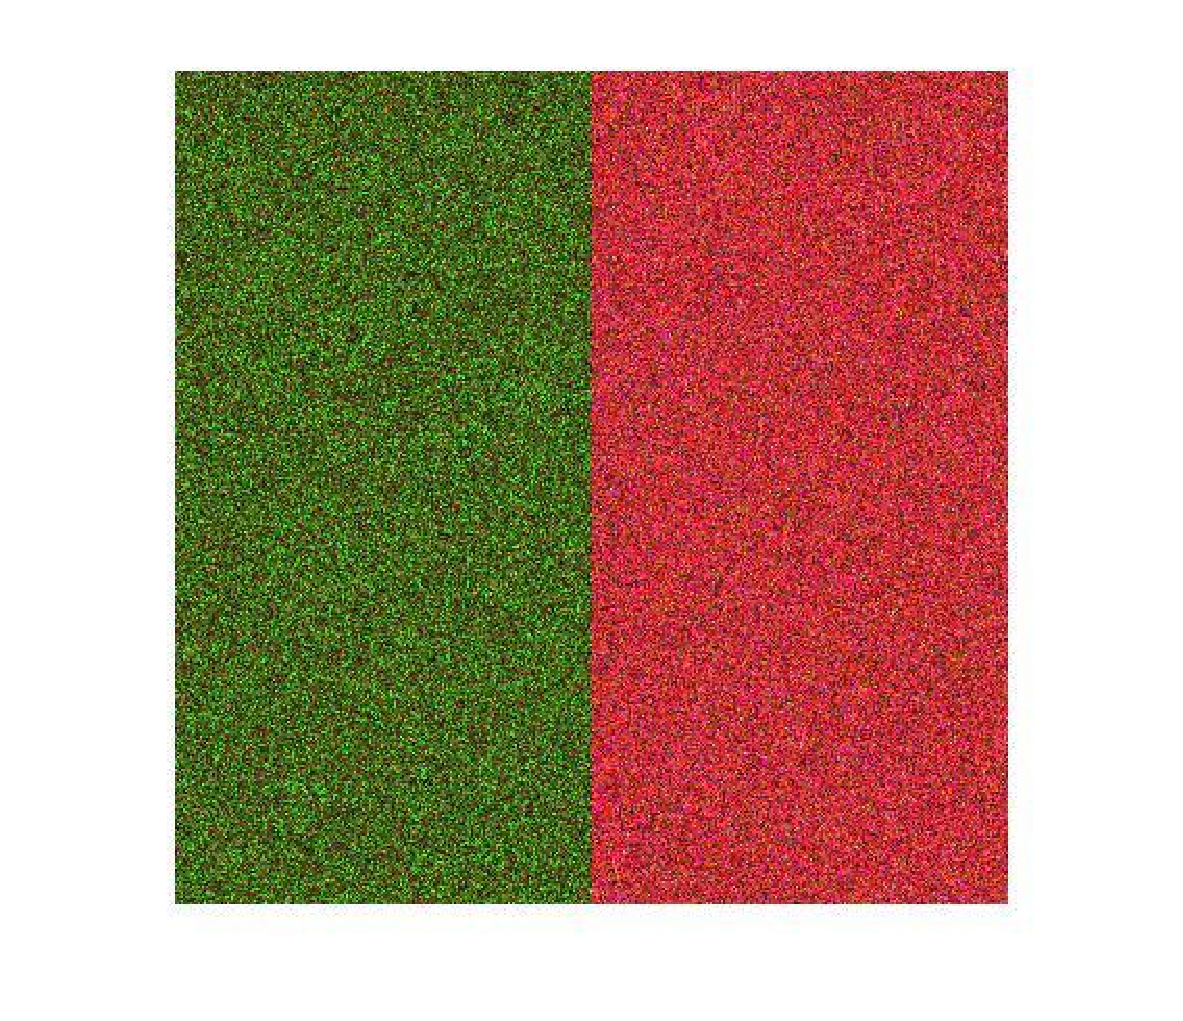
\includegraphics[width=5.0in]{phanton_nhfc_dec_pauli.pdf}
	\caption{Imagem simulada usando a decomposição de Pauli.}\label{fig:duas_folhas_nhfc}
\end{figure} 

A imagem simulada  usa $\Sigma_u$ e $\Sigma_f$ definidas por
\begin{equation}\label{matriz_sigma_nhfc_1}
	\hspace{2.75cm} \Sigma_{u}= \left[
\begin{array}{lll}
	962892             &19171 - 3579i&     -154638 + 191388i \\
	19171 + 3579i      &56707        &     -5798 + 16812i  \\
	-154638 - 191388i  &-5798 - 16812i&      472251 
\end{array}
\right],
\end{equation}
e
\begin{equation}\label{matriz_sigma_nhfc_2}
 \Sigma_{f}= \left[
\begin{array}{lll}
	360932            & 11050 + 3759i&   63896 + 1581i \\
	11050 - 3759i     & 98960       &   6593 + 6868i \\
	63896  - 1581i    & 6593  - 6868i&   208843
\end{array}
\right],
\end{equation}
onde os subescritos $u$ e $f$ definem respectivamente área urbana e floresta, podemos encontrar essas matrizes no artigo \citep{nhfc}.	

As informações sobre as evidências de bordas em imagens PolSAR podem ser obtidas pelos dados polarimétricos com respeito a cada canal de dados. Nesse trabalho usamos os canais de intensidades $I_{\text{hh}}$, $I_{\text{hv}}$ e $I_{\text{vv}}$ e será mostrado como obter informações das evidências de bordas combinando os canais através de diferentes distribuições densidades de probabilidades.   


\section{O método \textbf{MLE} aplicado à \textbf{PDF} univariada $\Gamma$}

Seja a \textbf{PDF} univariada $\Gamma$  
\begin{equation}\label{eq:univariada_gamma}
	f_{Z_{i}}(z_{i};\mu,L)=\frac{L^{L}z_{i}^{L-1}}{\mu^L\Gamma(L)} \exp(-L\frac{z_i}{\mu}), \\
\end{equation}
onde $i\in \{\textbf{hh}, \textbf{hv}, \textbf{vv}\}$, $\mu=\sigma_{i}^2$ a entrada $(i,i)$ da matriz $\Sigma$ e $z_{i}$ a entrada $(i,i)$ da matriz randômica $\mathbf{Z}$. Podemos verificar essa expressão em \citep{fnc, nhfc, hsbmp}.	 

A função densidade de probabilidade \eqref{eq:univariada_gamma} que modela o canal $(hh)$ aplicado nas matrizes de covariância com $L=4$ gerar a figura (\ref{fig:densidades_para_u_f_nhfc}). A representação gráfica da função de densidade para os respectivos $u$ e $f$ da matriz de covariância, representando área urbana e floresta. No gráfico definimos $\sigma^2_{hh}=962892$ e $\sigma^2_{hh}= 360932$. 

\begin{figure}[hbt]
	\centering
  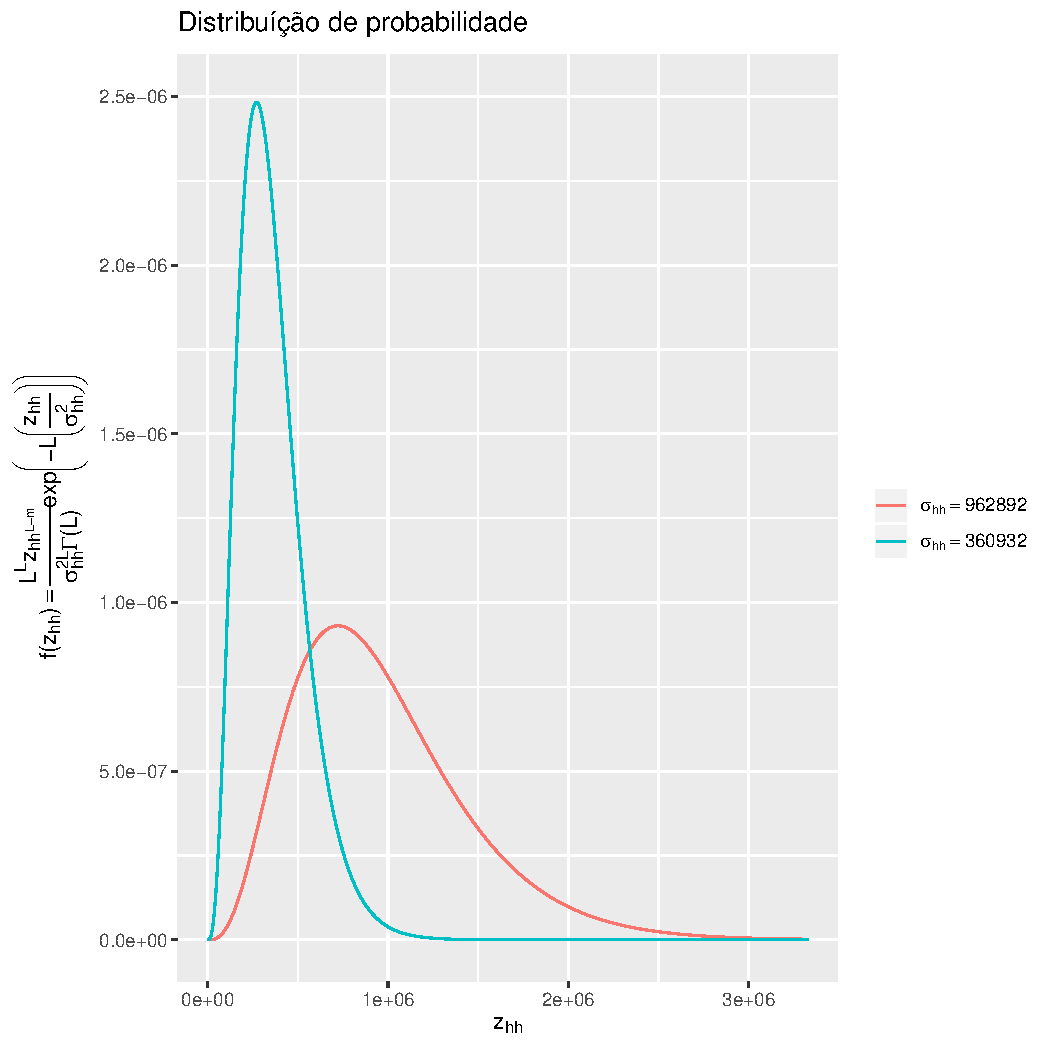
\includegraphics[scale = 0.7]{grafico_pdf_nhfc_2014_sigma_hh.pdf}
	\caption{Funções de densidade $\Gamma$ para dados simulados.}\label{fig:densidades_para_u_f_nhfc}
\end{figure}

	Em cada linha da imagem \eqref{fig:duas_folhas_nhfc} aplicamos o método \textbf{MLE} gerando a função de máxima verossimilhança $\ell(j)$. Nos gráficos \eqref{fig:funcao_l_gamma_nhfc_hh}, \eqref{fig:funcao_l_gamma_nhfc_hv} e \eqref{fig:funcao_l_gamma_nhfc_vv} são mostrados os canais de intensidades $I_{\text{hh}}$, $I_{\text{hh}}$ e $I_{\text{hh}}$ na linha horizontal fixa de número $200$. 
\begin{figure}[hbt]\label{fig:funcao_l_gamma_nhfc}
\minipage{0.5\textwidth}
  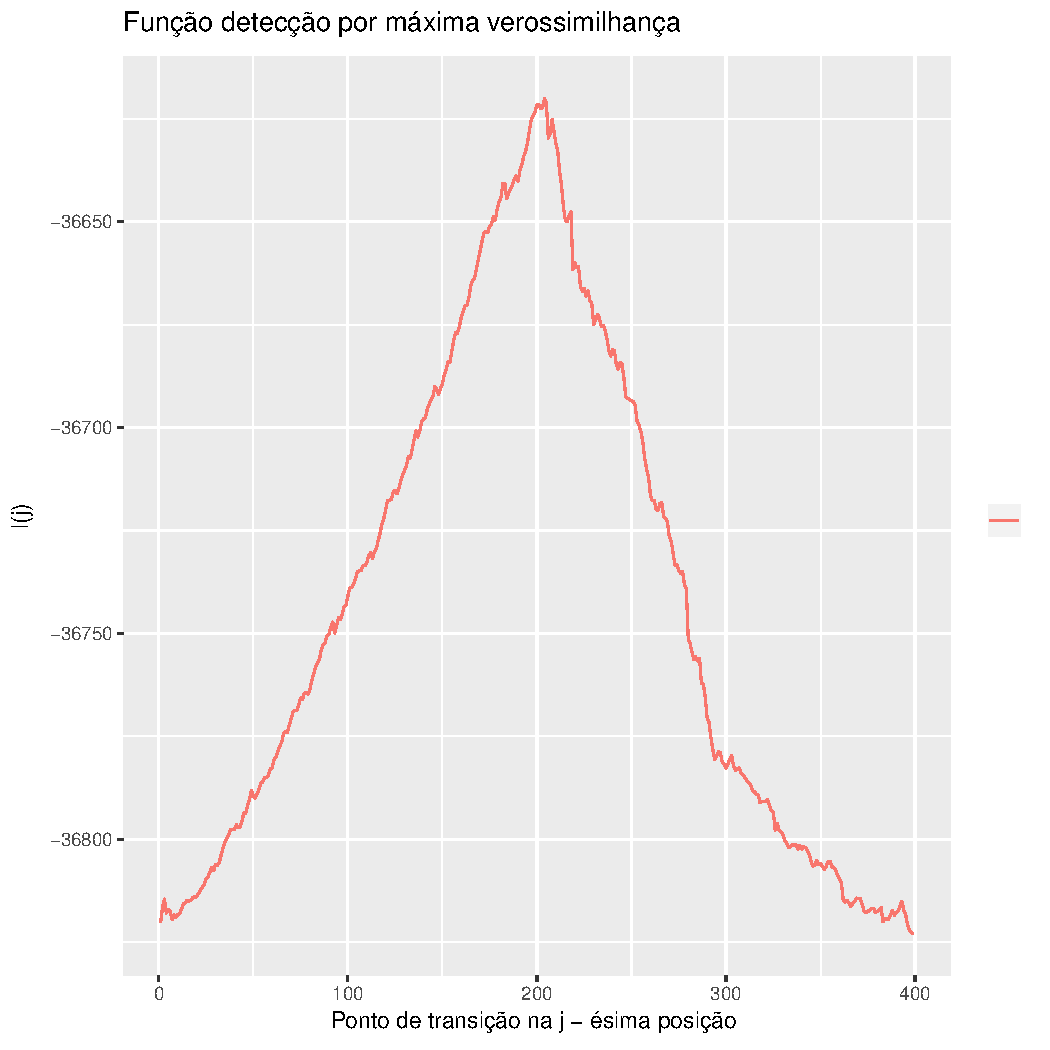
\includegraphics[width=\linewidth]{grafico_l_nhfc_2014_sigmahh.pdf}
	\caption{Função $\ell(j)$ para o canal $I_{HH}$}\label{fig:funcao_l_gamma_nhfc_hh}
\endminipage\hfill
\minipage{0.5\textwidth}
  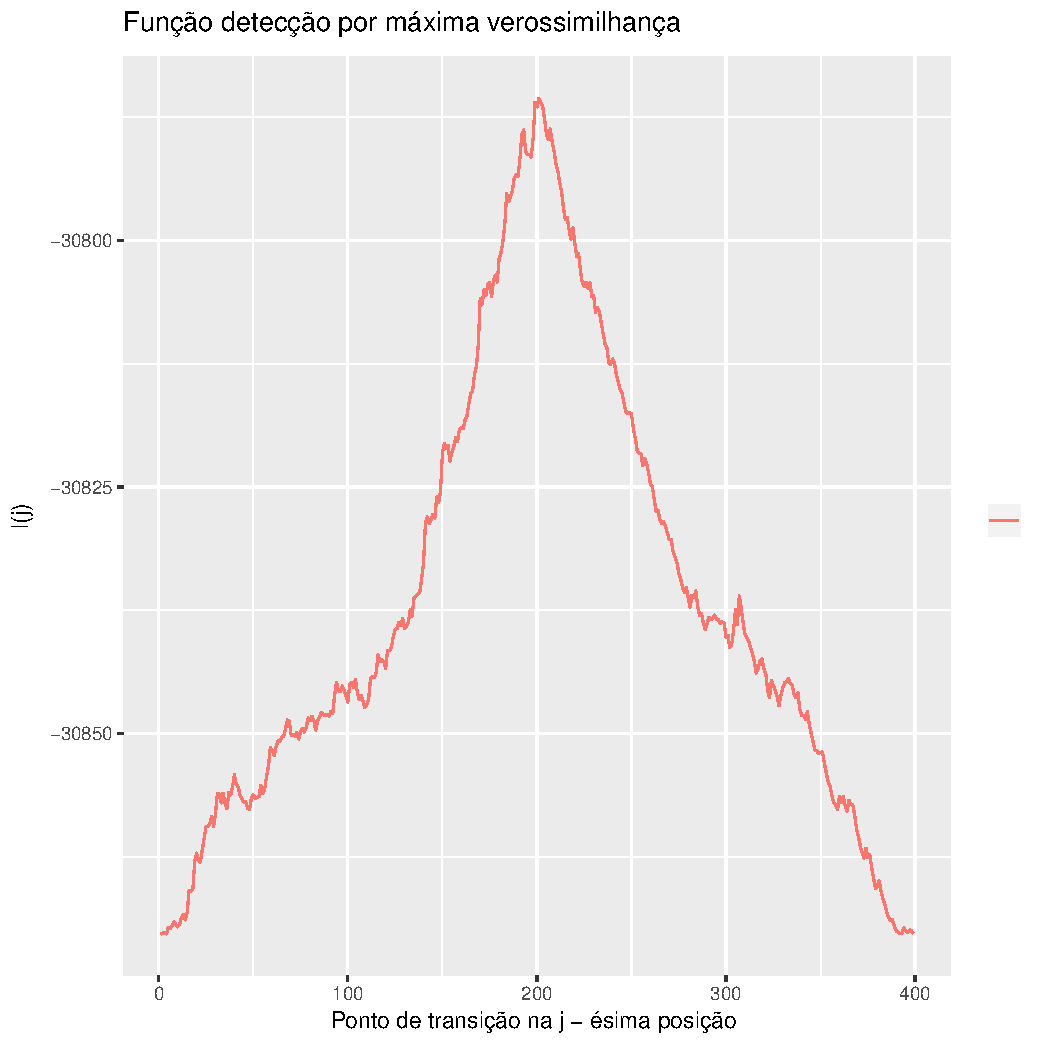
\includegraphics[width=\linewidth]{grafico_l_nhfc_2014_sigmahv.pdf}
	\caption{Função $\ell(j)$ para o canal $I_{HV}$}\label{fig:funcao_l_gamma_nhfc_hv}
\endminipage\hfill
\centering
\minipage{0.5\textwidth}
  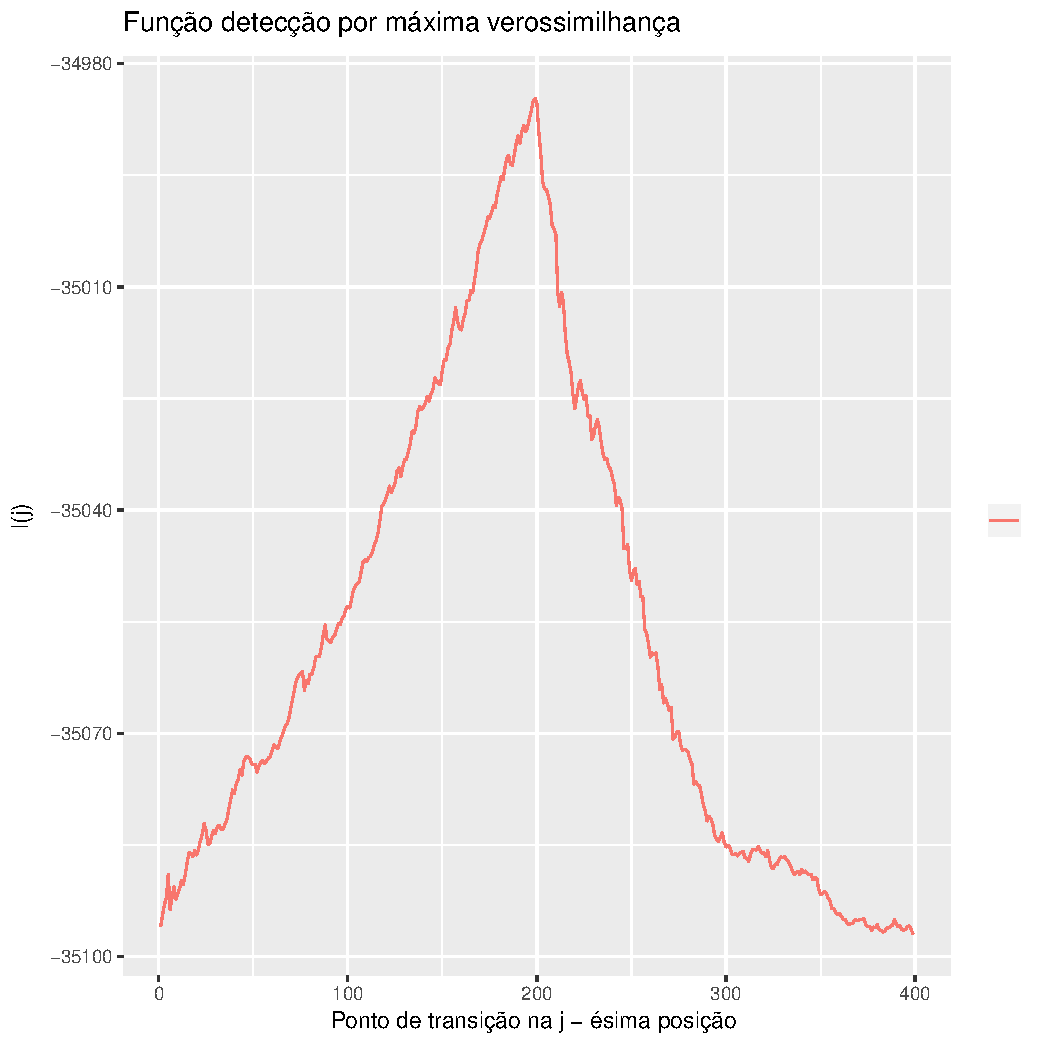
\includegraphics[width=\linewidth]{grafico_l_nhfc_2014_sigmavv.pdf}
	\caption{Função $\ell(j)$ para o canal $I_{VV}$}\label{fig:funcao_l_gamma_nhfc_vv}
\endminipage\hfill
\end{figure}

	Podemos notar que as funções não são deriváveis em muitos pontos, então os métodos de otimização que necessitam do cálculo da derivada, terão funcionamento comprometido, resolvemos esse problema usando o método Simulated Anneling Generalizado (GenSA) que podemos encontrar na referência \citep{xgsh}.
	
	O método GenSA mostrou-se competitivo com os métodos empregados no artigo \citet{nhfc}, para testar a acurácia do GenSA e fazer a comparação com os métodos aplicados no artigo, vamos usar a métrica encontrada no artigo \citep{nhfc} e proposta na referência \citep{fbgm}.
        
	O erro foi calculado gerando $400$ replicações da distribuição Wishart com duas amostras resultando em uma função $\ell(j)$  para cada replicação. Aplicando o GenSA para cada umas das $\ell(j)$ temos $400$ evidências de bordas ou pontos de transição. Se o ponto de borda referência construído está no pixel horizontal $200$, então o erro para cada replicação é o valor absoluto da diferença entre o ponto de borda referência e o valor estimado pelo método GenSA, ou seja,  
\begin{equation}\label{eq:erro}
\begin{array}{llll}
	E(r) &=& |200 - \hat{\jmath}(r)|, & 1\leq r \leq 400,  \\
\end{array}
\end{equation}
onde, $\hat{\jmath}(r)$ é o resultado da maximização de $\ell(j)$ pelo método GenSA na replicação $r$.

Usaremos frequências relativas para estimar a probabilidade de ter um erro menor que um número de pixeis. Denotando por $H(k)$ o número de replicações para qual o erro é menor que $k$ pixeis, então calculamos uma estimativa desta probabilidade por $f(k)=\frac{H(k)}{400}$. Nos testes realizados no trabalho variamos $k$ entre $1$ e $10$ e o algoritmo está descrito em detalhes na referência \citep{fbgm}. 

	A figura (\ref{fig:Probbilidade_erro}) mostra as probabilidades para a detecção de bordas quando aplicado o método GenSA nos canais $I_{hh}$, $I_{vh}$ e $I_{vv}$ da imagem mostrada na figura (\ref{cap_acf_fig01}). As 400 replicações para cada canal e sua respectiva evidência de borda estão nas figuras (\ref{cap_acf_fig07}),(\ref{cap_acf_fig08}) e (\ref{cap_acf_fig09}).  
\begin{figure}[hbt]
\centering
	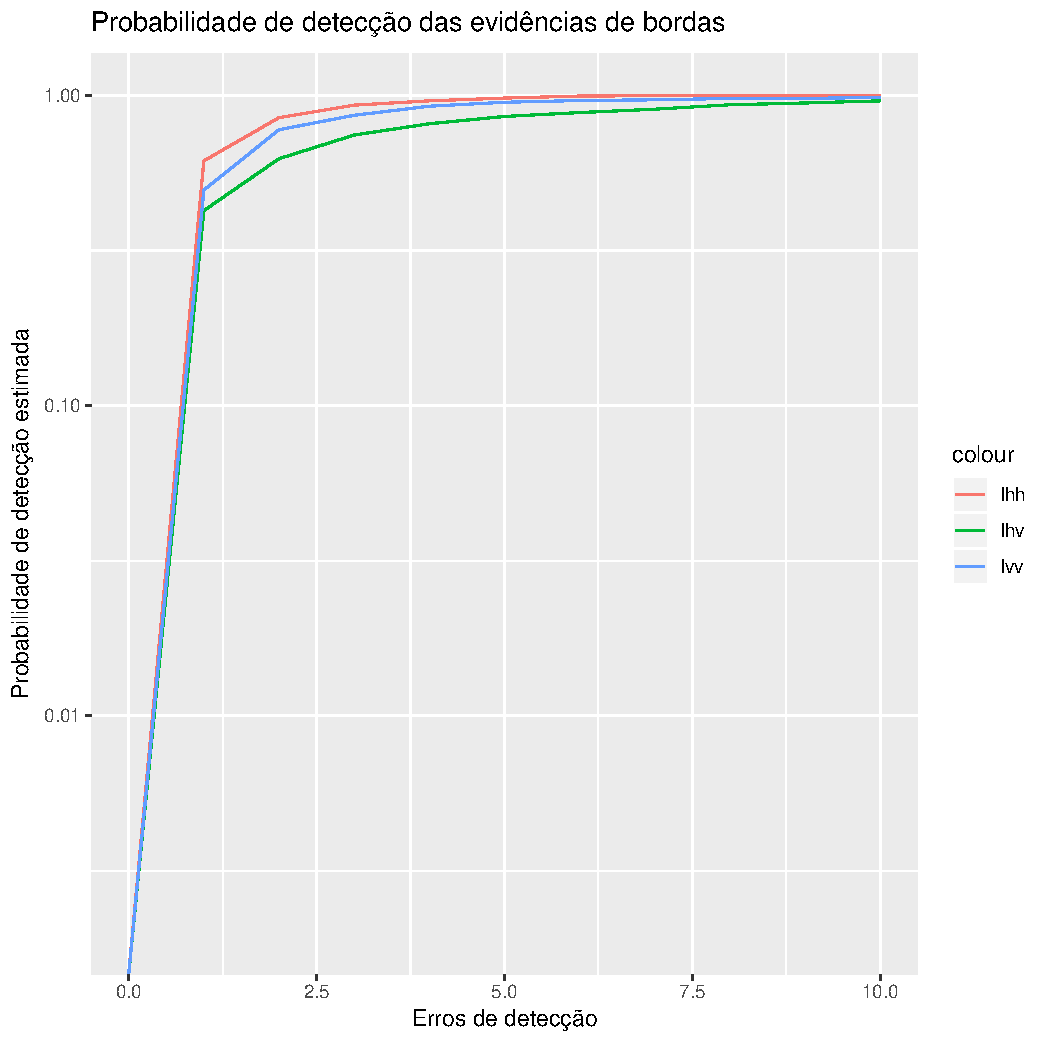
\includegraphics[width=5.0in]{metricas_ihh_ivh_ivv_nhfc.pdf}
	\caption{Probabilidade de detecção de borda estimada usando GenSA.}
\label{fig:Probbilidade_erro}
\end{figure}

\begin{figure}[hbt]
\minipage{0.475\textwidth}
\fbox{  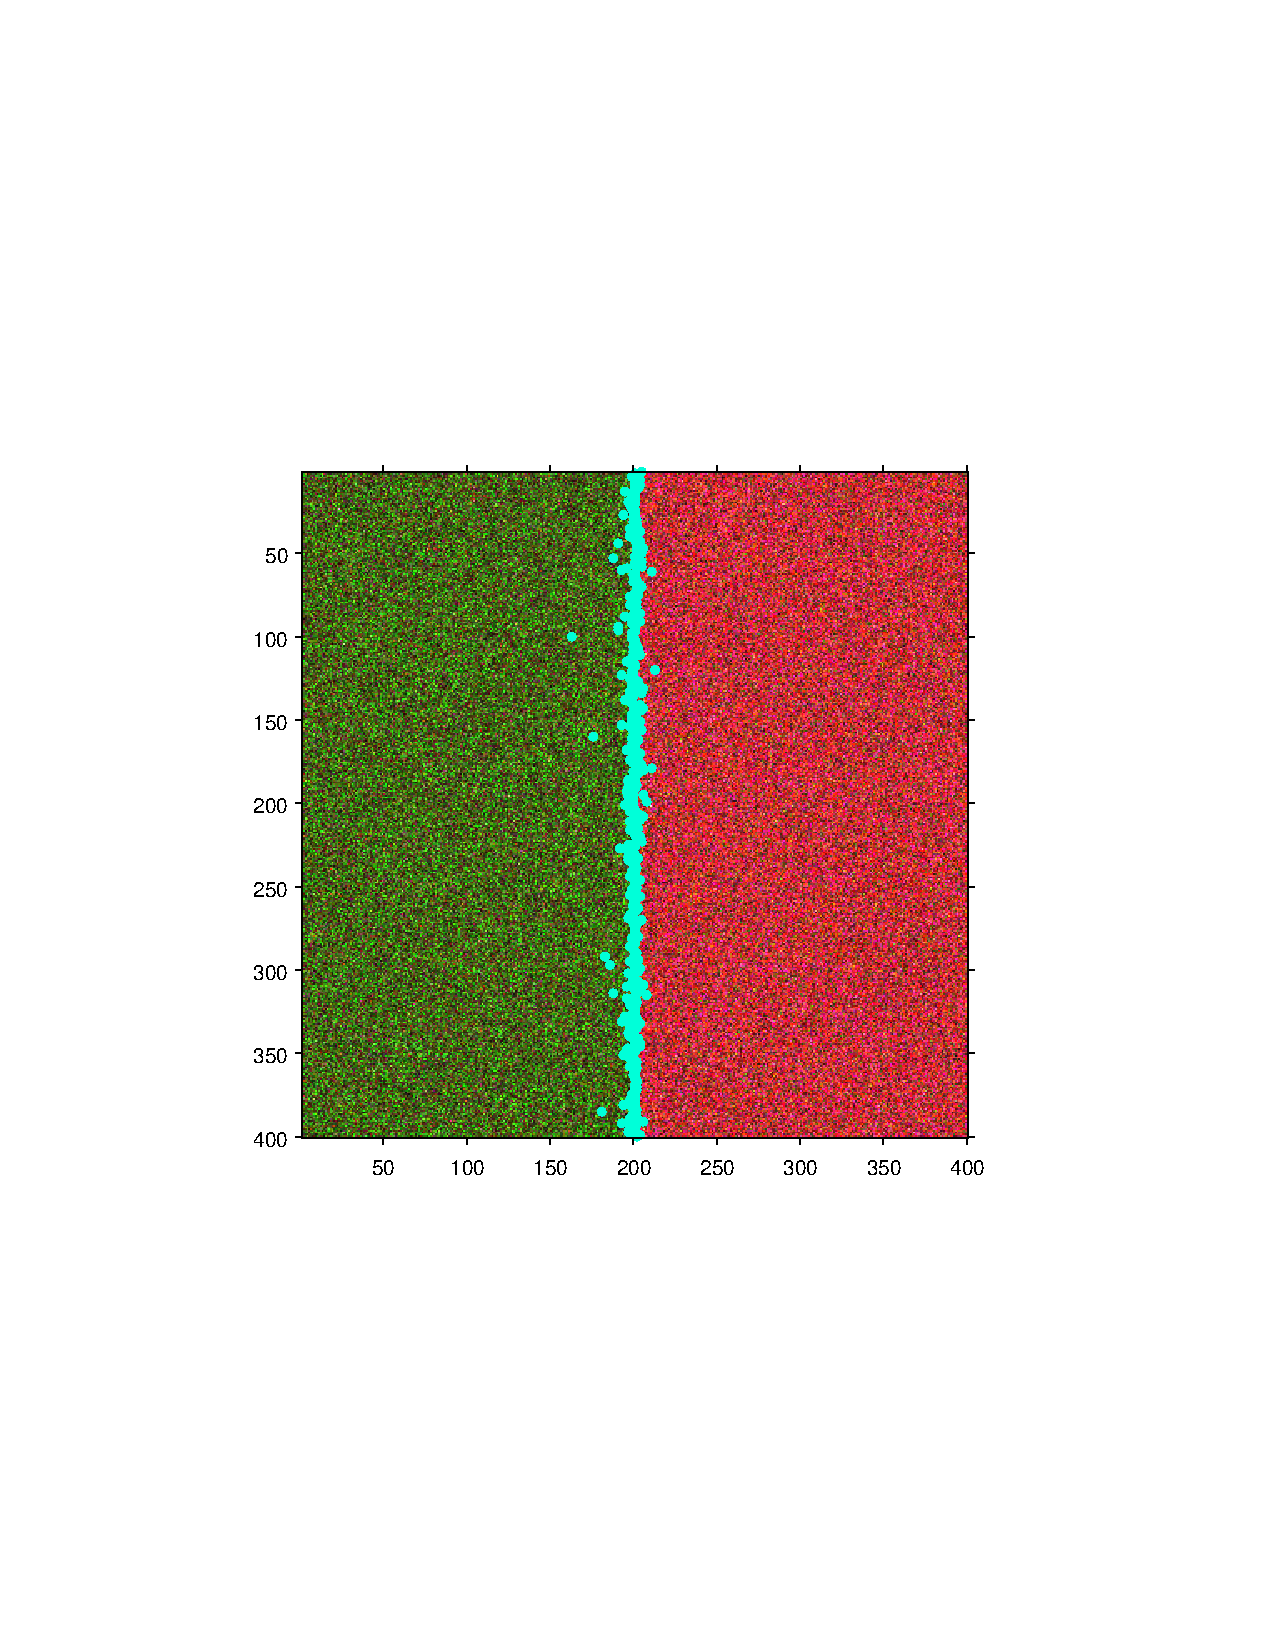
\includegraphics[width=\linewidth]{evidencia_duas_folhas_sim_hh}}
\caption{Evidências de bordas para o canal $I_{\text{hh}}$ na imagem simulada}\label{cap_acf_fig07}
\endminipage\hfill
\minipage{0.475\textwidth}
\fbox{ 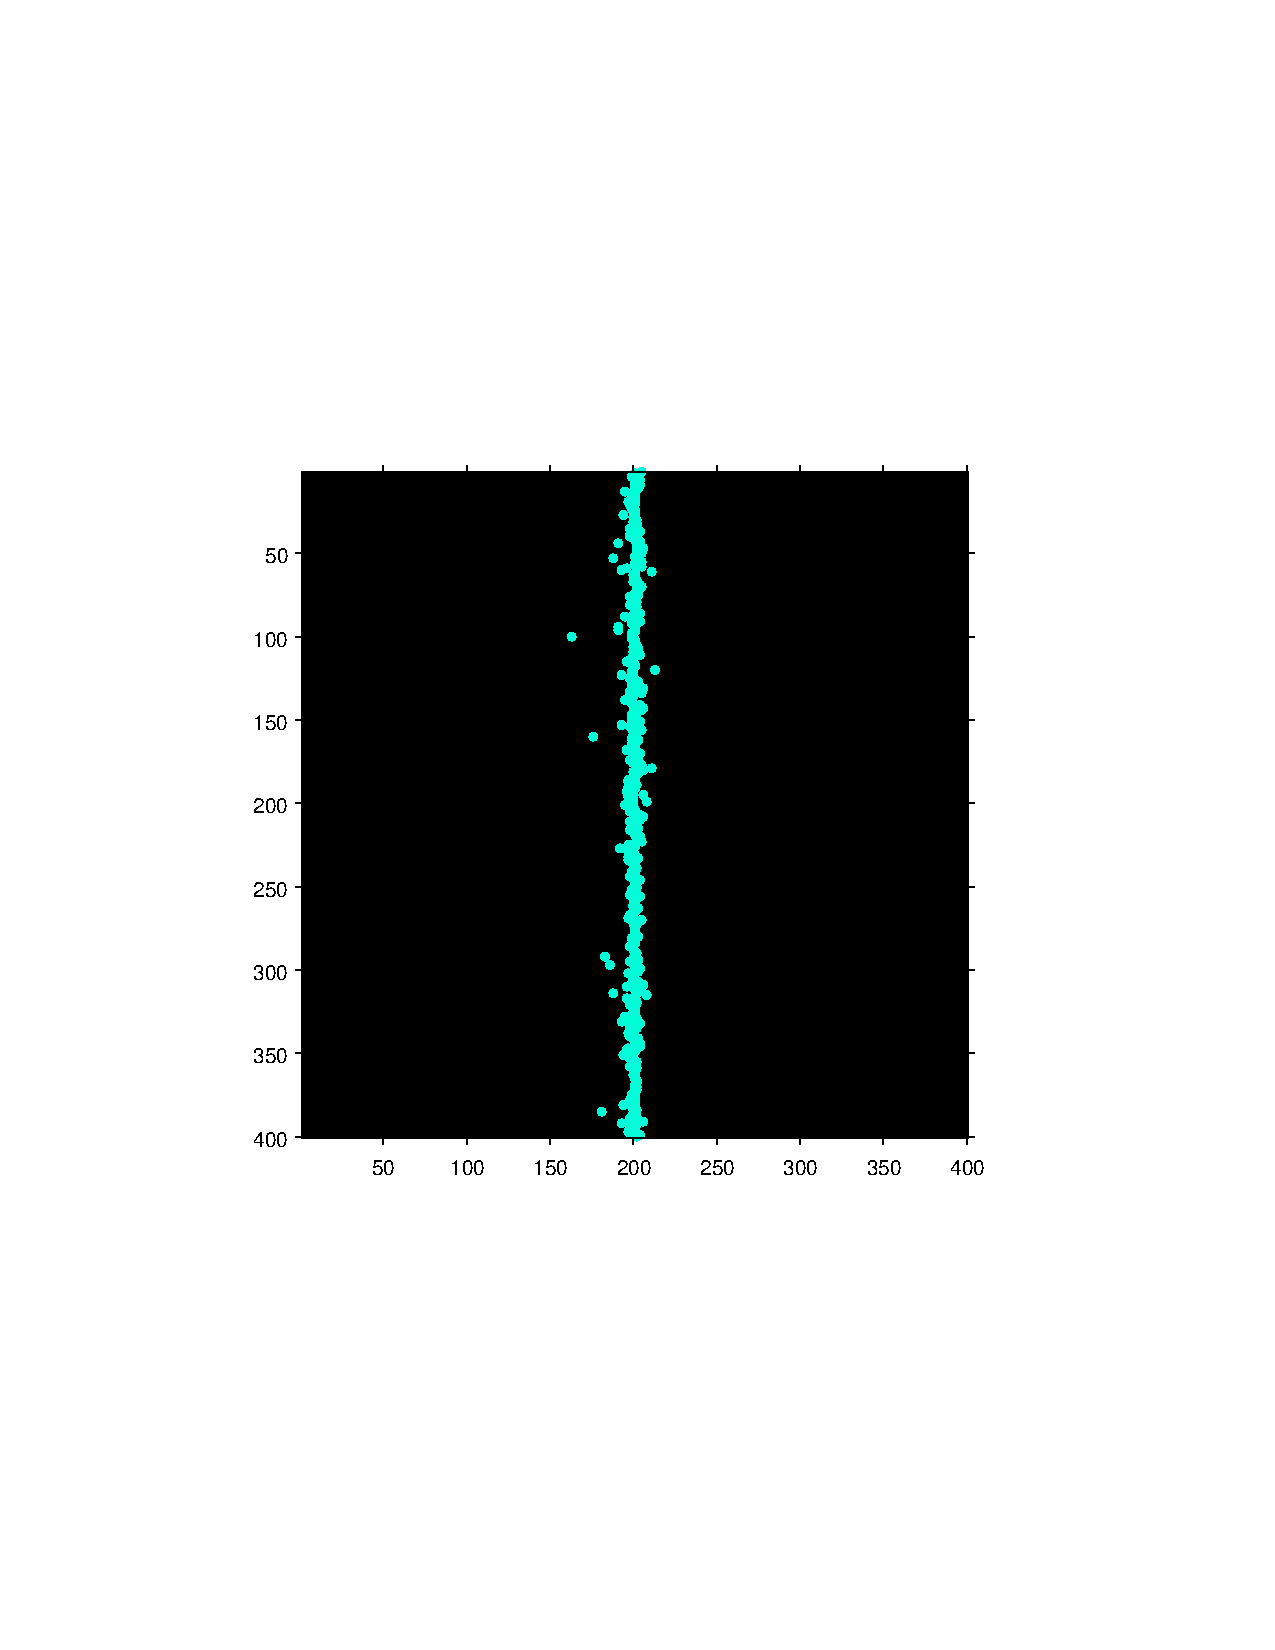
\includegraphics[width=\linewidth]{evidencia_duas_folhas_preto_hh}}
\caption{Evidências de bordas para o canal $I_{\text{hh}}$}\label{cap_acf_fig08}
\endminipage\hfill\\
\minipage{0.475\textwidth}
\fbox{  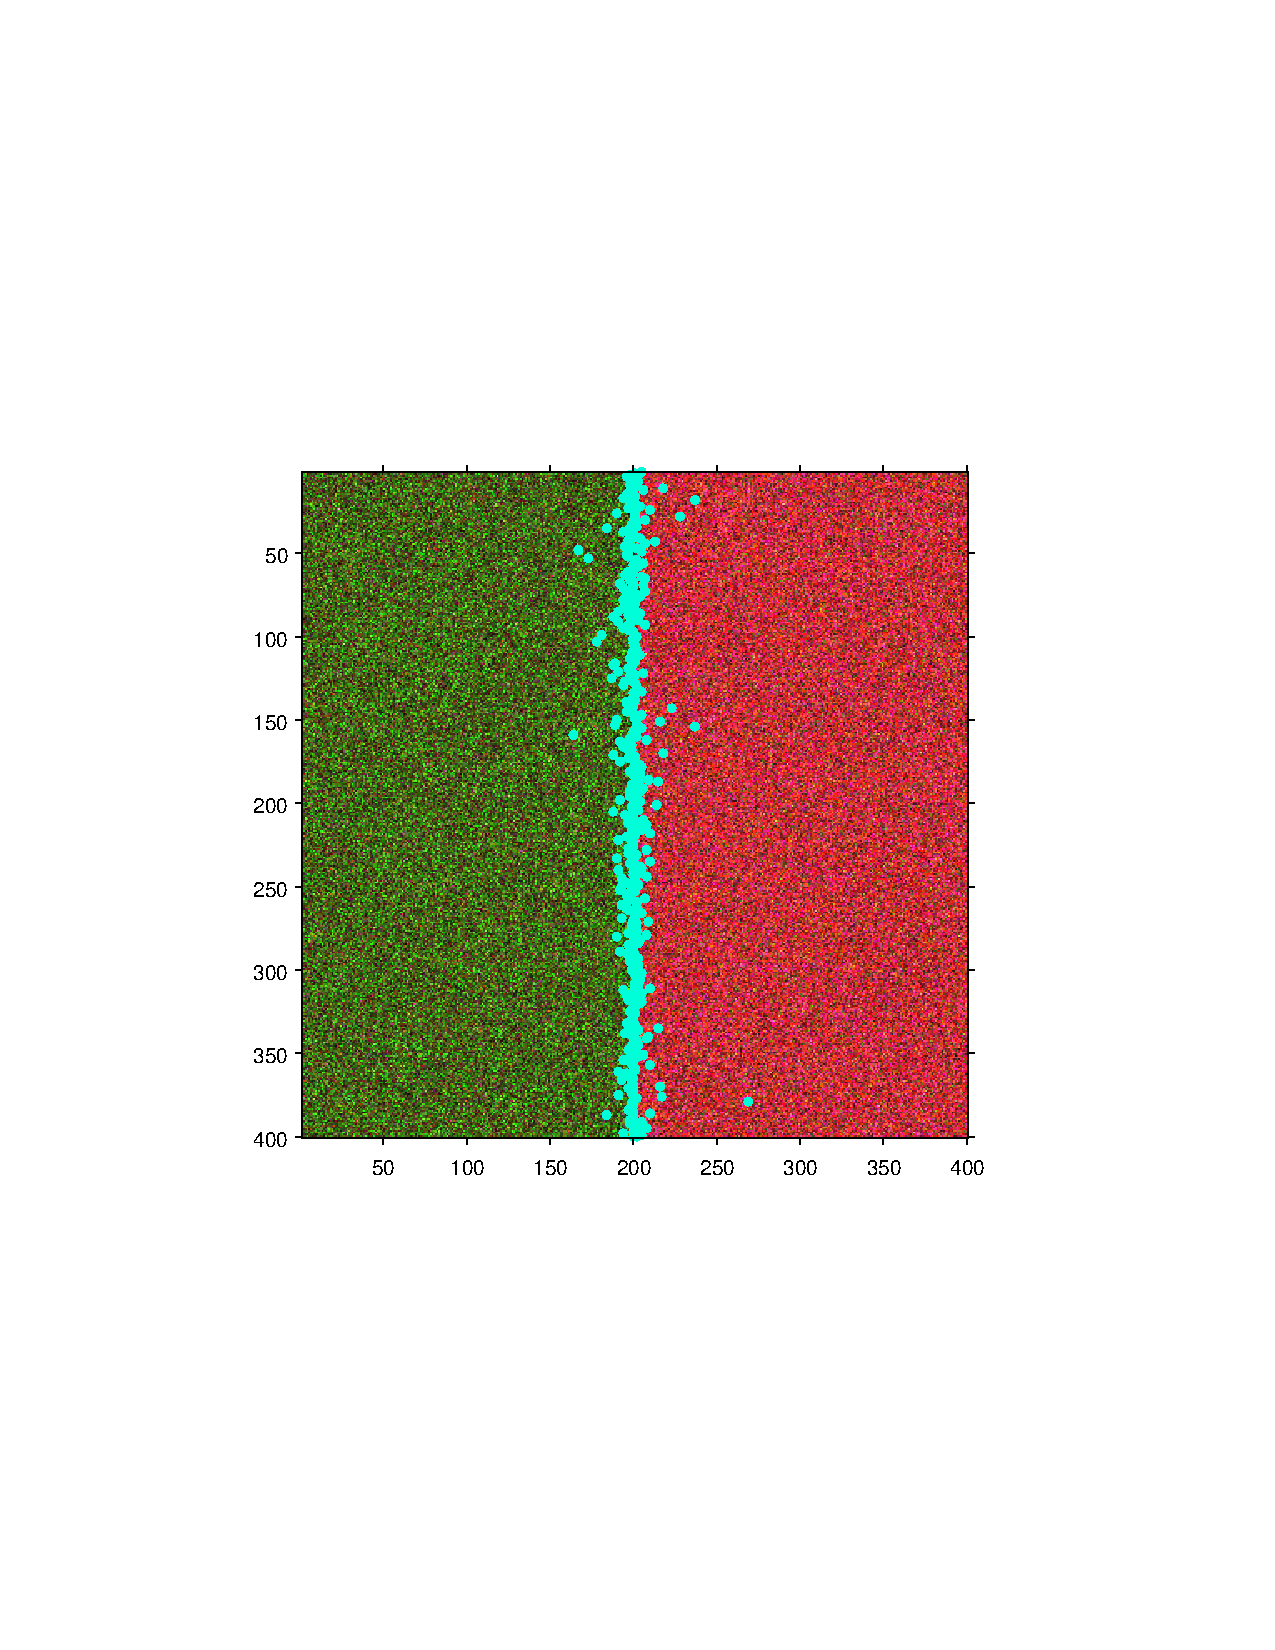
\includegraphics[width=\linewidth]{evidencia_duas_folhas_sim_hv}}
\caption{Evidências de bordas para o canal $I_{\text{hv}}$ na imagem simulada}\label{cap_acf_fig07}
\endminipage\hfill
\minipage{0.475\textwidth}
\fbox{ 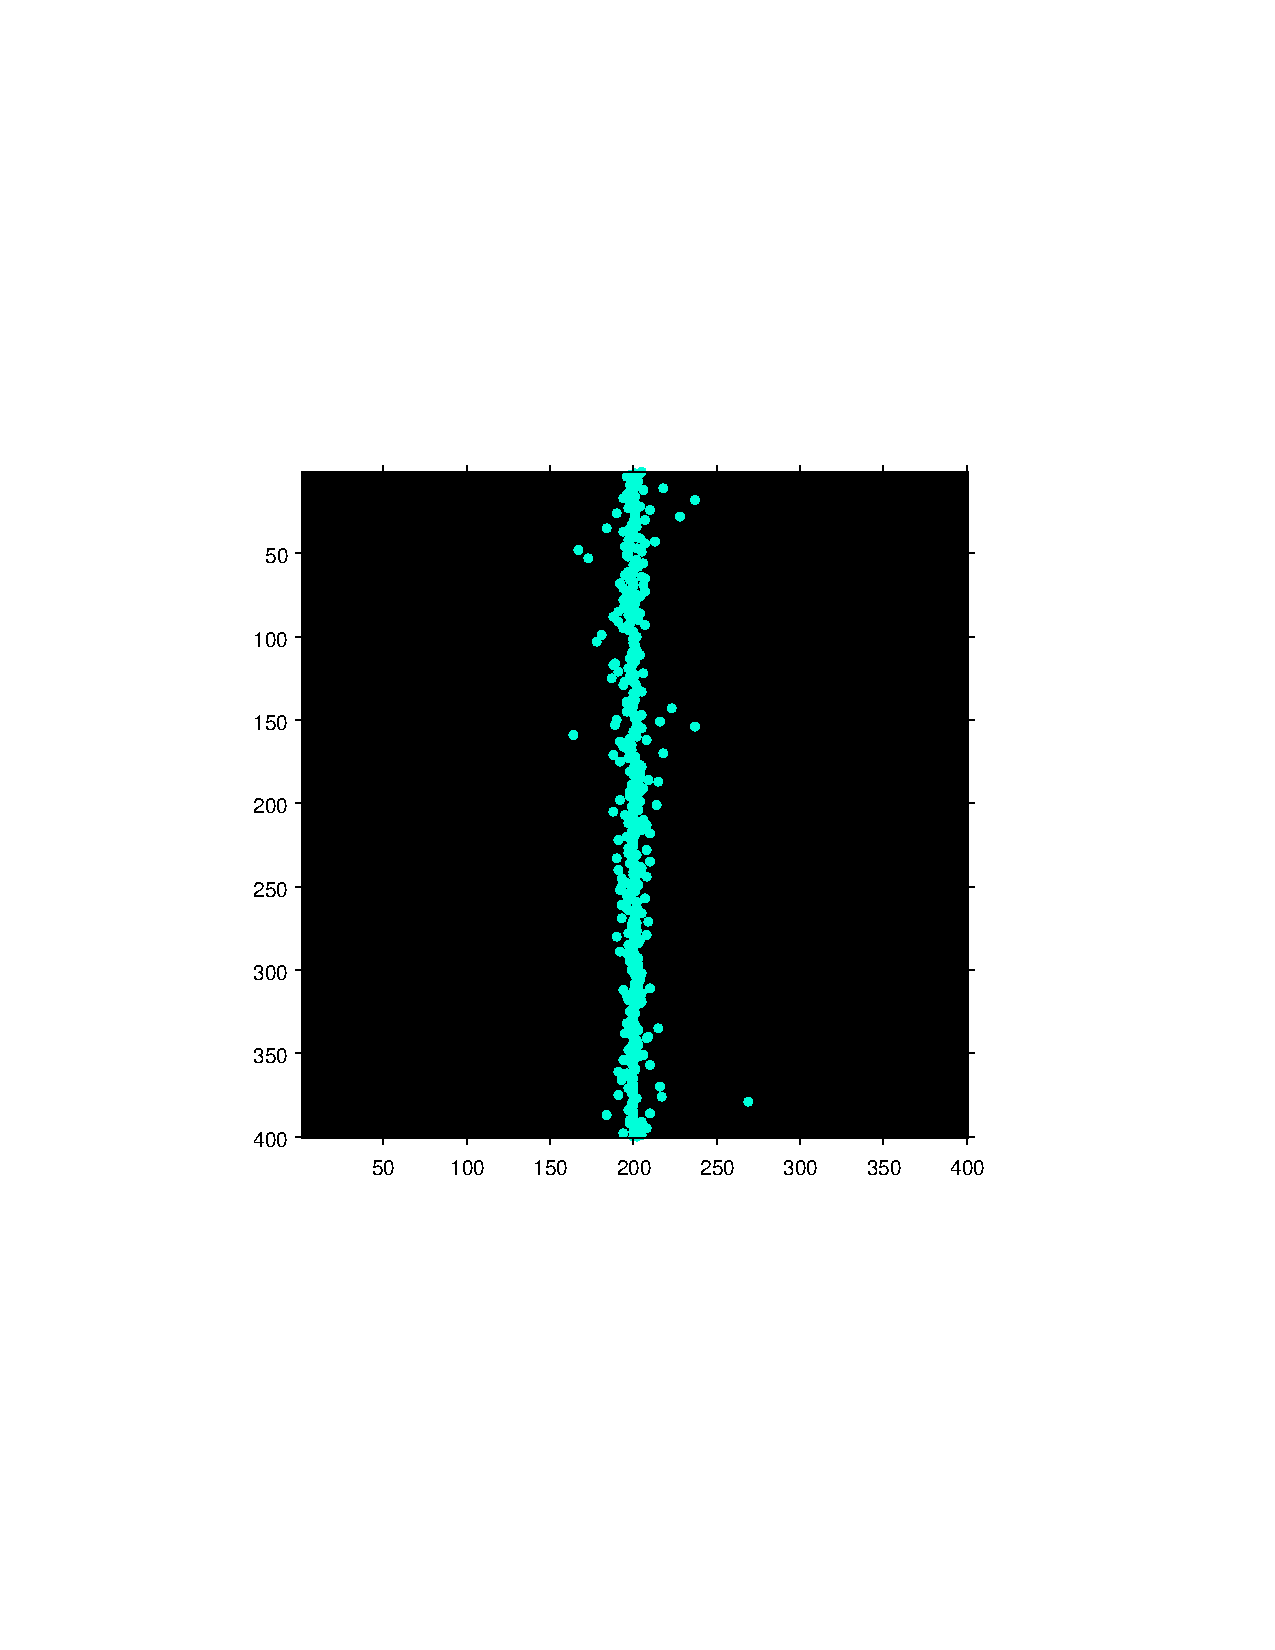
\includegraphics[width=\linewidth]{evidencia_duas_folhas_preto_hv}}
\caption{Evidências de bordas para o canal $I_{\text{hv}}$}\label{cap_acf_fig08}
\endminipage\hfill\\
\end{figure}

\begin{figure}[hbt]
\minipage{0.475\textwidth}
\fbox{  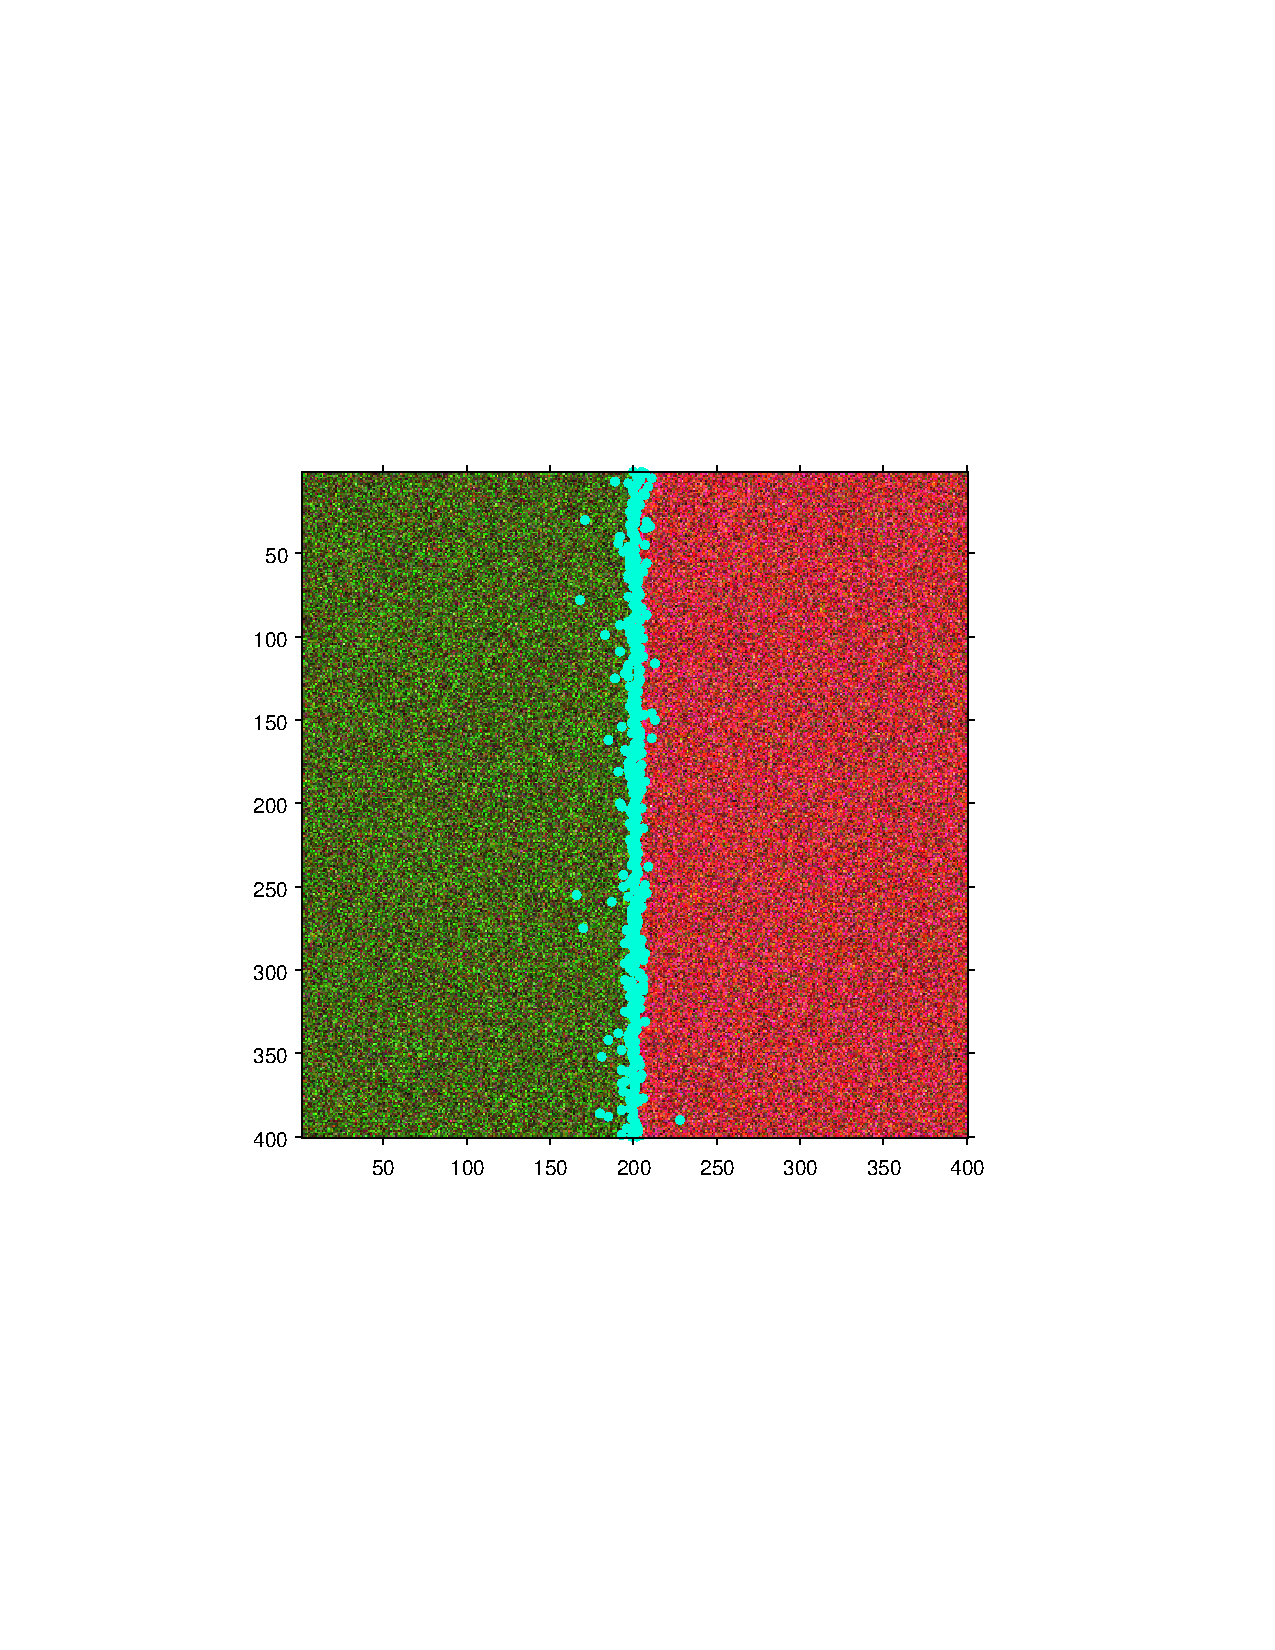
\includegraphics[width=\linewidth]{evidencia_duas_folhas_sim_vv}}
\caption{Evidências de bordas para o canal $I_{\text{vv}}$ na imagem simulada}\label{cap_acf_fig07}
\endminipage\hfill
\minipage{0.475\textwidth}
\fbox{ 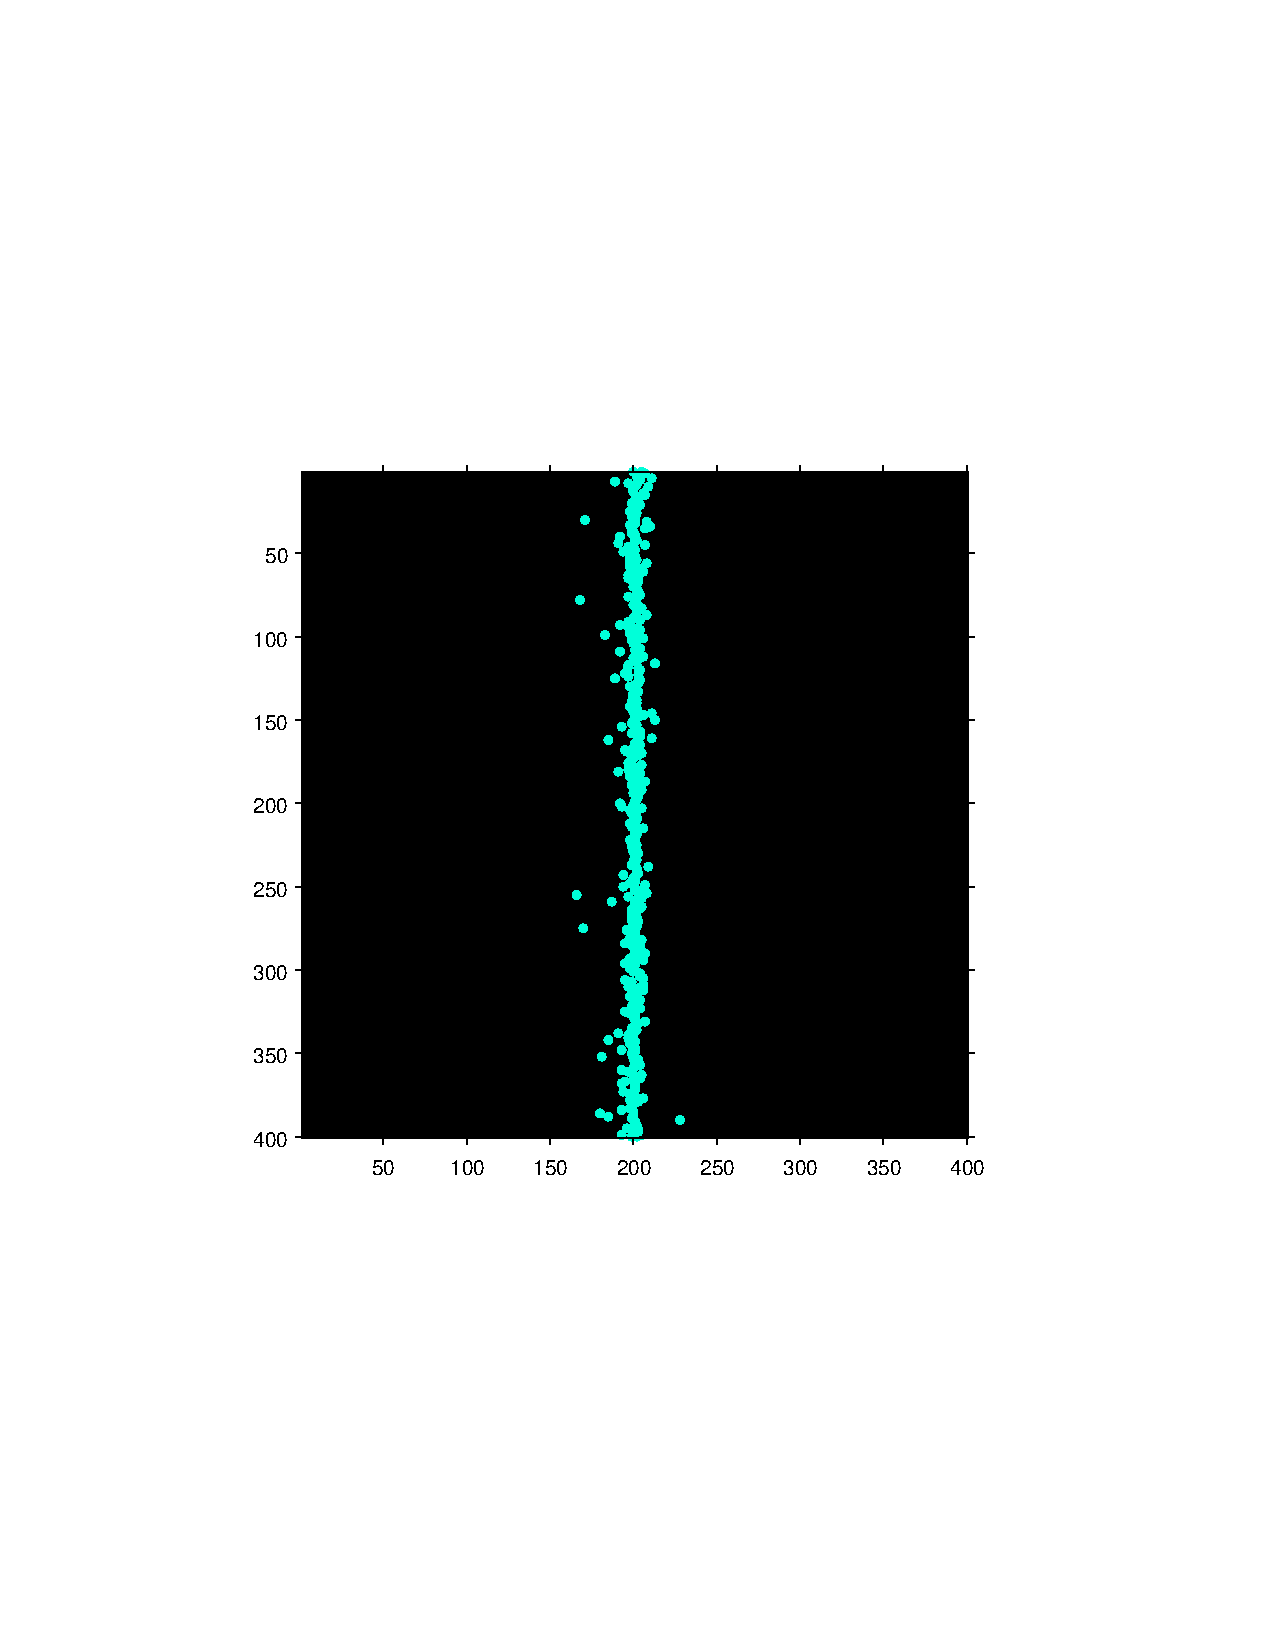
\includegraphics[width=\linewidth]{evidencia_duas_folhas_preto_vv}}
\caption{Evidências de bordas para o canal $I_{\text{vv}}$}\label{cap_acf_fig08}
\endminipage\hfill\\
\end{figure}

%\begin{figure}[hbt]
%\minipage{0.5\textwidth}
%  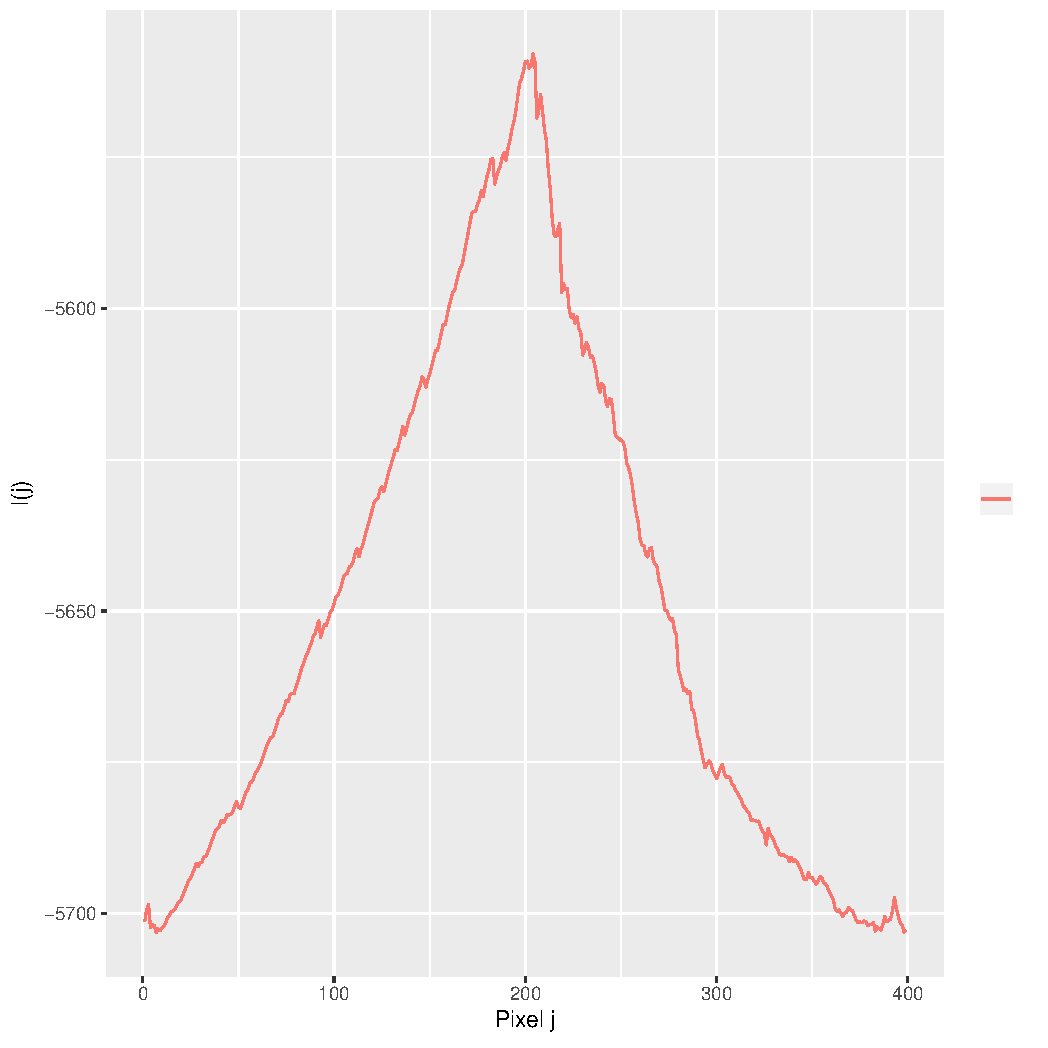
\includegraphics[width=\linewidth]{grafico_l_nhfc_2014_sigmahh_param_L_mu.pdf}
%	\caption{Função $l(j)$ para o canal $I_{HH}$}\label{cap_acf_fig04}
%\endminipage\hfill
%\minipage{0.5\textwidth}
%  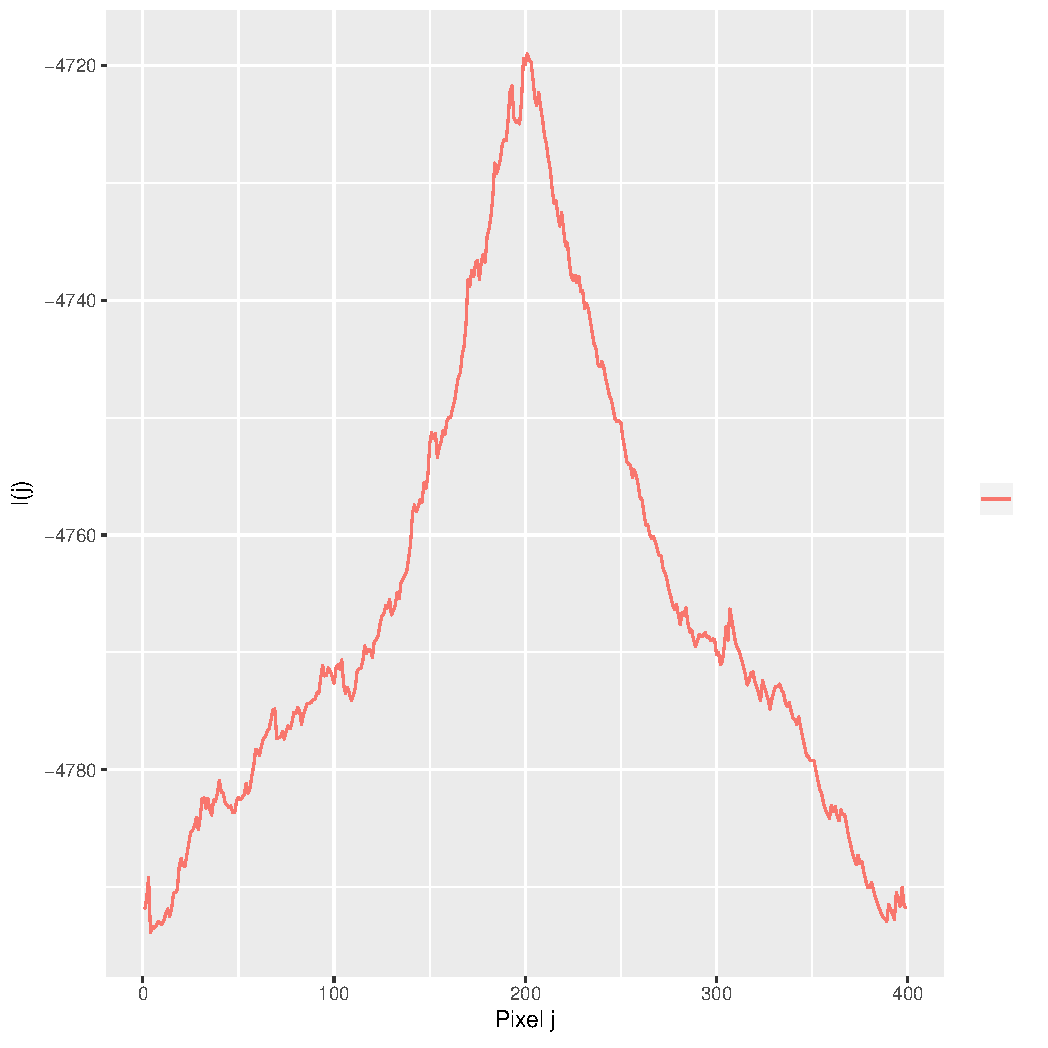
\includegraphics[width=\linewidth]{grafico_l_nhfc_2014_sigmahv_param_L_mu.pdf}
%	\caption{Função $l(j)$ para o canal $I_{HV}$}\label{cap_acf_fig05}
%\endminipage\hfill
%\centering
%\minipage{0.5\textwidth}
%  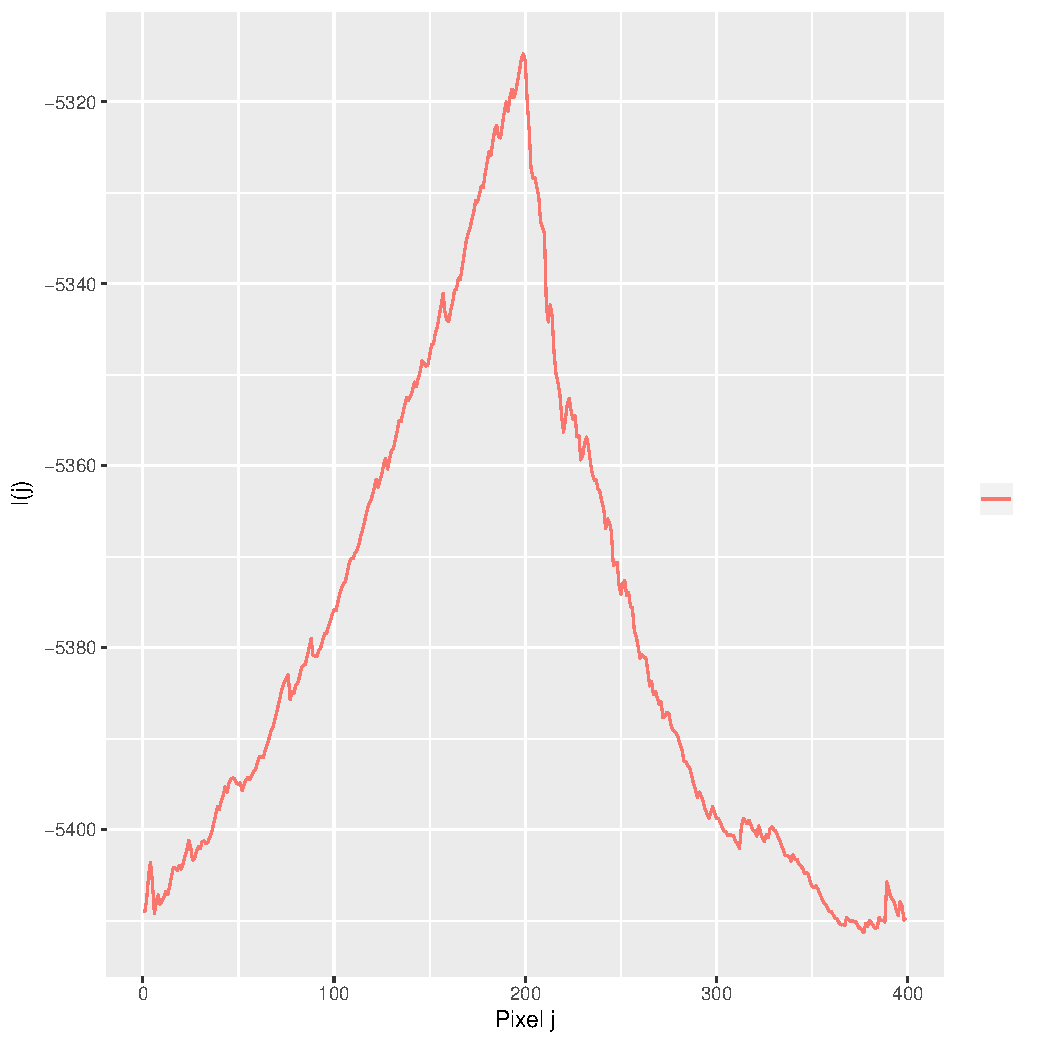
\includegraphics[width=\linewidth]{grafico_l_nhfc_2014_sigmavv_param_L_mu.pdf}
%	\caption{Função $l(j)$ para o canal $I_{VV}$}\label{cap_acf_fig06}
%\endminipage\hfill
%\end{figure}


